\chapter{X-ray Based Spectroscopy Methods}
\label{chapter:X-ray_Based_Spectroscopy_Methods}
In this chapter, the theoretical basics behind X-ray absorption spectroscopy (XAS) and resonant inelastic X-ray scattering (RIXS), which are the main experimental techniques used in this thesis, will be investigated. Both techniques can be used to investigate the local, element specific, electronic structure. This is of great advantage in comparison to conventional electronic spectroscopies like UV/Vis where the signals are broad and overlap with solvent bands, making it difficult to attribute them to distinct orbital contributions.
\section{Quantum Formulation of X-ray Interactions with Matter}
\label{sec:X-ray_Interaction_with_Matter}
X-rays interact with matter in through a variety of processes, each of them having different purposes in research or medical applications. Here, we will focus only on the interaction leading to X-ray absorption as this is the underlying process in the experimental techniques used in this thesis. This process involves an excitation of a core electron through the energy transfer of a photon to a bound electron, which is better known as the photoelectric effect \textcolor{red}{CITATION}. To calculate and understand the underlying transitions of this process, the quantum mechanical description of this interaction will be discussed in the following section.
\subsection{Basic Premise}
The quantum mechanical description of the photon-matter interactions has its roots in a paper by Kramers and Heisenberg in 1925 \cite{kramers1925streuung}, written just prior to the formal establishment of quantum theory. Their central idea was that the interaction between photons and matter can be treated as a weak perturbation of the matter's equilibrium state \cite{stohr2023nature}. As a results, photons act as a probe of the unperturbed ground state of matter. To model this perturbation, a Hamiltonian is required describing the interaction of an electromagnetic field with the electron charge and spin.  A derivation of the complete interaction Hamiltonian can be found in the literature \cite{stohr2023nature}. For simplicity, we consider only the most dominant terms which are given as:
\begin{equation}
    \hat{H}_{int} = \underbrace{\frac{e^{2}}{2m_{e}}\hat{A}^{2}}_{\substack{\text{Thomson}\\\text{scattering}}}
    +\underbrace{\frac{e}{m_{e}}\hat{p}\cdot\hat{A}}_{\substack{\text{photoelectric}\\\text{transitions}}} , 
    \label{eq:tot_hamiltonian}
\end{equation}
where $e$ is the elementary charge, $m_{e}$ the electron mass, $\hat{A}$ is the time-dependent vector potential and $\hat{p}$ the momentum, given in operator form. The vector potential $\hat{A}(\textbf{r},t) = \hat{A}^{ab} + \hat{A}^{em}$ can cause absorption (and thereby photon destruction) or emission (through photon creation) \cite{stohr2023nature}. If the term depends linearly on $\hat{A}$, it describes processes in which a photon is either created or annihilated, but not both simultaneously. In contrast, if the term depends quadratically on $\hat{A}$, it allows for both photon creation and annihilation, corresponding to scattering processes. \\
The essence of the description of electronic excitations lies in the assumption that the system is mostly time independent and that the time evolution can be approximate by a weak perturbation. This concept is used in time-dependent perturbation theory where the total Hamiltonian can be separated into two parts $\hat{H} = \hat{H}_{0} + \hat{H}'$ where the  $\hat{H}'$ acts a weak time-dependent perturbation of the stationary $\hat{H}_{0}$. This is justified here as the interaction process with a single photon is so fast (<\SI{1}{\atto\second}) that it is not affected by other atomic effects witch occur on longer timescales. This relative speed comparison is the same concept as in the Born-Oppenheimer approximation \cite{born_oppenheimer1927}. Using the quantization of the electromagnetic field introduced by Dirac in 1927 \cite{dirac1927quantizationEM}, this leads to the Kramers-Heisenberg-Dirac perturbation theory.
\subsection{The Kramers-Heisenberg-Dirac Formula}
According to the Kramers-Heisenberg-Dirac (KHD) perturbation theory, the time-dependent electromagnetic field induces a transitions from an initial state $\ket{i}$ to a final state $\ket{f}$. Both states include electronic and photonic components, and the transition can be envisioned as proceeding through a multiple steps. First, the electronic and photon parts of the system are decoupled, so that the electronic ground state evolves according to the time-independent Hamiltonian. Second, the interaction takes place, when the electronic state is perturbed by the interaction Hamiltonian $\hat{H}_{int}$ (see eq. \ref{eq:tot_hamiltonian}) generating a new state $\ket{f}$. This transition can be written as $\braket{f|\hat{H}_{int}|i}$. Third, the electronic excited state evolves again according to the time-independent Hamiltonian. In second order, the transition is made through an intermediate state $m$, which gives $\braket{f|\hat{H}_{int}|m}\braket{m|\hat{H}_{int}|i}$. The analogue formulation can be made for higher order of perturbations, however we stop here after the second order term, which can be then formulated as the Kramers-Heisenberg-Dirac (KHD) formula, which is the starting point of quantitative calculation of electronic X-ray processes under the assumption of the Born-Oppenheimer approximation \cite{stohr2023nature}. The transition probability $\mathcal{W}_{if}$ from a state $i$ to a state $f$ is given as:
\begin{equation}
    \mathcal{W}_{if} = \frac{2\pi}{\hbar}\left|\underbrace{\braket{f|\hat{H}_{int}|i}}_{1^{st}}+\underbrace{\sum_{m}\frac{\braket{f|\hat{H}_{int}|m}\braket{m|\hat{H}_{int}|i}}{\mathcal{E}_{i}-\mathcal{E}_{m}}}_{2^{nd}}\right|^{2} \rho\left(\mathcal{E}_{f}\right)\delta\left(\mathcal{E}_{f}-\mathcal{E}_{i}\right),
    \label{eq:Kramers-Heisenberg-Dirac}
\end{equation}
where $\hat{H}_{int}$ is the interaction Hamiltonian, $\ket{i}$, $\ket{m}$ and $\ket{f}$ are the wavefunctions of the initial, intermediate and final state with their respective energies $\mathcal{E}_{i}$, $\mathcal{E}_{m}$ and $\mathcal{E}_{f}$, $\rho(\mathcal{E}_{f})$ is the density of states of final states, and $\delta$ is the Dirac $\delta$-function conserving the energy. The first term of the matrix element is better known as "Fermi's golden rule" \cite{fermi1932}. The second term describes transitions from the initial state $i$ to the finale state $f$ over a range of possible intermediate states $m$. Based on this equation, we will discuss in the following sections the transition rate and cross-sections of the processes in X-ray absorption spectroscopy and Resonant inelastic X-ray scattering.
\begin{figure}[H]
    \centering
    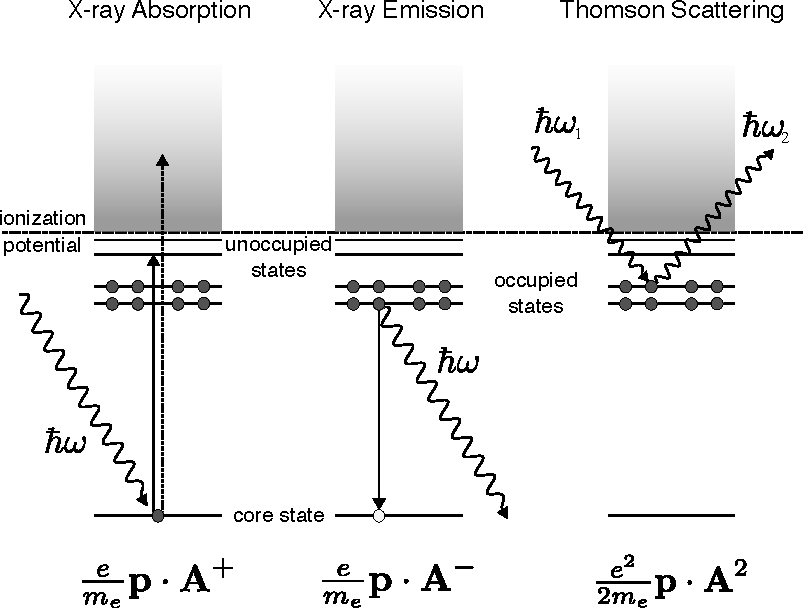
\includegraphics[width=0.8\linewidth]{Figures/first_order_interaction_processes.pdf}
    \caption{Schematic of the first order quantum mechanical process upon interaction of X-rays with matter. Electrons are shown as filled circles, holes as open circles. The operators for the processes are shown below.}
    \label{fig:Overview_first_order_processes}
\end{figure}
\noindent
Using only the first order term of the KHD equation (eq. \ref{eq:Kramers-Heisenberg-Dirac}), leads to the quantum mechanical description of X-ray absorption, X-ray emission and X-ray Thomson scattering, illustrated in Figure \ref{fig:Overview_first_order_processes}, along with their respective interaction Hamiltonian. In X-ray absorption or emission the X-ray photon is absorbed (destroyed) or emitted (created). This is described by the destruction operator $\hat{A}^{+}$ or the creation operator $\hat{A}^{-}$, respectively. Thomson scattering does neither destroys or creates photons and can occur as an elastic or inelastic process. In the following, we will discuss the underlying concepts of X-ray absorption in greater detail.
\section{X-ray Absorption Spectroscopy}
The strongest interaction of X-rays with matter is X-ray absorption. In this process, the incident electric field couples to a core electron, resulting in the absorption of the photon and the transfer of its energy to the electron, which is thereby promoted to an unoccupied level or ejected from the system if the incidence energy is larger than the ionization potential. Both processes are depicted in Figure \ref{fig:Overview_first_order_processes} (solid and dashed line). Measuring the photon energy dependent cross section, which is the sum of all photoemission cross sections of orbitals with energy lower than the photon energy, is the main essence of X-ray absorption spectroscopy (XAS). This cross section changes smoothly with photon energy, decreasing with increasing photon energy (shell specific photoemission cross section increases with photon energy), and exhibits sharp so-called absorption edges, where the photon energy matches resonant excitations.
\begin{figure}[H]
    \centering
    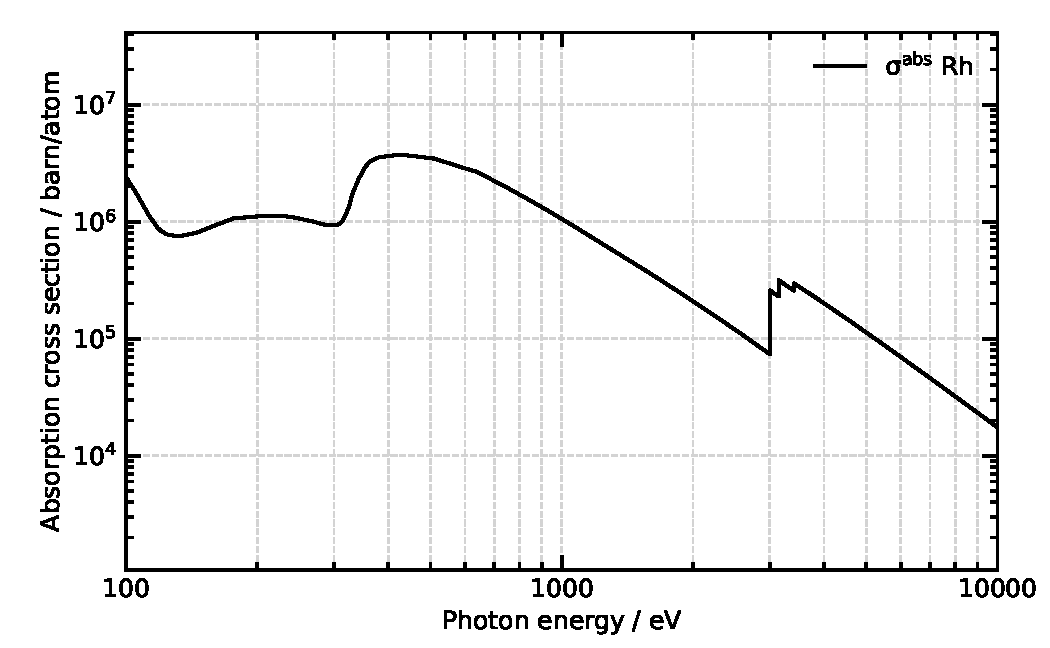
\includegraphics[width=\linewidth]{Figures/Cross_section_Rh.pdf}
    \caption{Energy dependent X-ray absorption cross section for Rh. The cross sections were calculated from atomic scattering factors from literature \cite{henke1993x}.}
    \label{fig:Rh_Cross_section}
\end{figure}
\noindent
Excitations which exceed resonance excitations in energy can arise from multi-electron excitations, and in the case of molecular or condensed matter due to back scattering of photoelectrons from neighboring atoms. This part of the spectrum is called extended X-ray absorption fine structure (EXAFS) and will not be discussed here in detail. We will focus here on the resonant near absorption fine structure (NEXAFS) part of XAS, which corresponds to excitations of core electrons to empty valence orbitals, which makes it sensitive to the bonding environment. \\\
To get back to the quantum mechanical description, we utilized the first order term of the KHD equation (\ref{eq:Kramers-Heisenberg-Dirac} which gives the transition rate for X-ray absorption:
\begin{equation}
    \mathcal{W}_{if}^{abs} = \frac{2\pi}{\hbar}\left|\braket{f|\hat{H}_{int}|i}\right|^{2} \rho\left(\mathcal{E}_{f}\right)\delta\left(\mathcal{E}_{f}-\mathcal{E}_{i}\right).
    \label{eq:XAS_transition_rate}
\end{equation}
with $\hat{H}_{int} = e \textbf{r}\cdot\hat{E}$, which is a combination of the dipole operator $e\ \textbf{r}$ and the field operator $\hat{E}$ which can analogously to vector potential $\hat{A}$ can destroy ($\hat{E}^{+}$) or create ($\hat{E}^{-}$) photons. Until here, the electric field operator $\hat{E}$ depends on the wave vector \textbf{k}, according to  
\begin{equation}
    E(\textbf{r}, t) = E_{0}e^{i\left(\textbf{k}\cdot\textbf{r}-\omega t\right)},
    \label{eq:electric_field}
\end{equation}
where $\textbf{r}$ is the position vector, $\omega$ is the angular frequency and $t$ is the time. In the dipole approximation, the exponential can be expanded as 
\begin{equation}
   e^{i\textbf{k}\cdot\textbf{r}} = 1 + i\textbf{k}\cdot\textbf{r} + \cdots \simeq 1, 
    \label{eq:exponential_expansion}
\end{equation}
which makes the electric field uniform across the interaction region. As a result, the interaction Hamiltonian $\hat{H}_{int}$ reduces to the dipole operator, and dipole-allowed transitions -- subject to the selection rule $\Delta L = \pm 1$ -- dominate the transitions. To get the cross section for the X-ray absorption process, the transition rate per unit time $\mathcal{W}_{if}^{abs}$ has to be normalized by the incident photon flux $\Phi_{0}$
\begin{equation}
    \sigma^{abs} = \frac{\mathcal{W}_{if}^{abs}}{\Phi_{0}} \qquad \mathrm{with} \qquad \Phi_{0}=\frac{c n_{0}}{V}=\frac{2\epsilon_{0}cE^{2}_{0}}{\hbar\omega},
    \label{eq:XAS_cross_section}
\end{equation}
where $\epsilon_{0}$ is the electric field constant, $c$ the speed of light and $E_{0}$ the amplitude of the electric field. The photon flux $\Phi$ can be imagined as the number of photons $n_{0}$ flowing with the speed of light $c$ through a specific volume $V$.\\
Following the creation of a core hole through photon absorption, the system stabilizes by spontaneously filling the vacancy. The core hole is filled by an electron form a higher energy level which results in the release of energy. This energy can be either transferred to a valence electron which is ejected from the atom (Auger-Meitner decay) or by the emission of a photon (fluorescence). The ratio of these two decay channels varies with the atomic number $Z$, with Auger-Meitner decay being favored for lighter elements and fluorescence for heavier elements \cite{kotani2001resonant}. The final states reached through these two channels are distinct, meaning that they do not interfere. Consequently, the individual decay rates for X-ray emission $\Gamma^{X}$ and for Auger-Meitner decay $\Gamma^{AM}$ can be summed to give total decay rate $\Gamma$:
\begin{equation}
    \Gamma = \Gamma^{X} + \Gamma^{AM}
    \label{eq:decay_rate_XAS}
\end{equation}
The finite lifetime of the electronic excited states results in a natural broadening, also known as lifetime broadening. This is a result of the Heisenberg uncertainty principle \cite{heisenberg1927anschaulichen}, which, in its energy-time relation, refers the lifetime to its uncertainty in energy
\begin{equation}
    \Delta E \Delta t \geq  \frac{\hbar}{2},
    \label{eq:Heisenberg_uncertainty}
\end{equation}
where $\Delta E$ is the uncertainty in energy and $\Delta t$ is the uncertainty in time. As the decay of electronic excited state occurs exponentially in time, the corresponding lineshape are Lorentzian and $\Gamma$ represents the Lorentzian FWHM. 
\section{Resonant Inelastic X-ray Scattering}

\section{Time-resolved Spectroscopy}
\section{X-ray Sources}
\label{sec:X-ray_sources}
\subsection{Synchrotron Radiation}
\subsection{Free Electron Lasers}
